\documentclass[letterpaper,12pt]{article}

\usepackage[letterpaper,margin=1in]{geometry}
\usepackage{fancyhdr}
\usepackage{amsmath,amssymb}
\usepackage{enumerate}
\usepackage{xcolor}
\usepackage{tikz}


\pagestyle{fancy}
\fancyhf{}
\lhead{Problem Set 1}
\rhead{STAT 314 -- Statistical Theory}
\renewcommand{\headrulewidth}{0.4pt}
\setlength{\headheight}{14.5pt}

\begin{document}


\noindent
\begin{minipage}{0.5\textwidth}
    \raggedright
    \textbf{Name:} Daryll Jewel D. Lanic
\end{minipage}%
\begin{minipage}{0.5\textwidth}
    \raggedleft
    \textbf{Section:} BSAPMATH 3-2
\end{minipage}

\vspace{1.5em}

\begin{center}
	{\LARGE\bfseries Problem Set 1}\par
	\vspace{0.5em}
	{\large Probability Models, Distributions, Joint Distributions, Transformations, and Order Statistics}\par
\end{center}

\vspace{2em}

\noindent\textbf{Problem 1. Constructing a Distribution from Constraints [12 points]}
\vspace{0.5em}

A continuous random variable $X$ has probability density function
\[
f_X(x) = 
\begin{cases} 
a + bx, & 0 < x < 2, \\ 
0, & \text{otherwise}, 
\end{cases}
\]
and
\[\mathbb{E}(X) = \frac{7}{6}.\]

\begin{enumerate}[(a)]
    \item Using only the defining properties of a probability density function and the given expectation, derive a system of equations for $a$ and $b$.
    \vspace{0.5em}
    \begin{list}{}{} \item[] 
        \textbf{Answer:}
        
        \textbf{For the first equation,}
        By the definition of a valid probability density function (PDF),
        \[
        \int_{-\infty}^{\infty} f_X(x) \, dx = 1
        \]
        Since $f_X(x) = a + bx$ for $0 < x < 2$ and $0$ otherwise, then
        \begin{align*}
        \int_{0}^{2} (a + bx) \, dx = 1 
        &\implies \left[ ax + \frac{b}{2}x^2 \right]_{x=0}^{x=2} = 1 \\
        &\implies a(2) + \frac{b}{2}(2)^2 - a(0) - \frac{b}{2}(0)^2 = 1 \\
        &\implies 2a + 2b = 1.
        \end{align*}

        \textbf{For the second equation,}
        
        By the definition of expectation,
        \[
        \mathbb{E}(X) = \int_{-\infty}^{\infty} x f_X(x) \, dx = \frac{7}{6}
        \]
        Then,
        \begin{align*}
        \int_{0}^{2} x(a + bx) \, dx = \frac{7}{6}
        &\implies \left[ \frac{ax^2}{2} + \frac{bx^3}{3} \right]_{x=0}^{x=2} = \frac{7}{6} \\
        &\implies \frac{a(2)^2}{2} + \frac{b(2)^3}{3} - \frac{a(0)^2}{2} - \frac{b(0)^3}{3} = \frac{7}{6} \\
        &\implies \frac{4a}{2} + \frac{8b}{3} = \frac{7}{6} \\
        &\implies 2a + \frac{8b}{3} = \frac{7}{6}.
        \end{align*}
    \end{list}
    
    \item Solve the system and determine the values of $a$ and $b$.
    \item Prove that the resulting function is a valid probability density function on its stated support.
    \vspace{0.5em}
    \begin{list}{}{} \item[] 
        \textbf{Answer:}
        
        With $a = \frac{1}{4}$ and $b = \frac{1}{4}$, the resulting probability density function is
        \[
        f_X(x) = 
        \begin{cases} 
        \frac{1}{4} + \frac{1}{4}x = \frac{1}{4}(1 + x), & 0 < x < 2, \\ 
        0, & \text{otherwise}. 
        \end{cases}
        \]
        To prove that $f_X(x)$ is a valid probability density function, we verify the two required axioms:
        \begin{enumerate}[1.]
            \item \textbf{Non-negativity:} $f_X(x) \ge 0$ for all $x \in \mathbb{R}$.
            \item \textbf{Normalization:} $\int_{-\infty}^{\infty} f_X(x) \, dx = 1$.
        \end{enumerate}

        \vspace{0.5em}
        \textbf{For the Non-negativity condition ($f_X(x) \ge 0$):}
            \quad For $x \in (0, 2)$: Since $x > 0$, we have $1 + x > 1 > 0$. Thus,
            \[f_X(x) = \frac{1}{4}(1 + x) > 0.\]
            \quad For $x \notin (0, 2)$:
            \[f_X(x) = 0 \ge 0.\]
        \noindent Thus, $f_X(x) \ge 0$ holds for all $x \in \mathbb{R}$.

        \vspace{0.5em}
        \textbf{For the Normalization condition ($\int_{-\infty}^{\infty} f_X(x) \, dx = 1$):}
        
        Evaluating the total area under $f_X(x)$,
        \begin{align*}
        \int_{-\infty}^{\infty} f_X(x) \, dx 
        &= \int_{0}^{2} \left( \frac{1}{4} + \frac{1}{4}x \right) dx \\
        &= \left[ \frac{1}{4}x + \frac{1}{8}x^2 \right]_{0}^{2} \\
        &= \left( \frac{1}{4}(2) + \frac{1}{8}(2)^2 \right) - \left( \frac{1}{4}(0) + \frac{1}{8}(0)^2 \right) \\
        &= \left( \frac{1}{2} + \frac{4}{8} \right) - 0 \\
        &= \frac{1}{2} + \frac{1}{2} \\
        &= 1.
        \end{align*}
        
        Since both conditions---non-negativity ($f_X(x) \ge 0$ for all $x \in \mathbb{R}$) and normalization ($\int_{-\infty}^{\infty} f_X(x) \, dx = 1$)---are satisfied, $f_X(x)$ is formally proven to be a valid probability density function on its stated support.
    \end{list}
    \item Derive the complete piecewise cumulative distribution function $F_X(x)$.
    \item Derive $\mathbb{E}(X^2)$ and $\text{Var}(X)$.
    \item Let $m$ denote the median of $X$. Determine $m$ exactly and decide whether $m$ is less than, equal to, or greater than $\mathbb{E}(X)$. Justify your conclusion analytically.
\end{enumerate}
\vspace{1.5em}

\subsection*{Problem 2. Distribution Identification Through\\ Moment-Generating Functions \hfill \mdseries[12 points]}
Let $X_1, X_2, \dots, X_n$ be independent Bernoulli random variables satisfying
\[P(X_i = 1) = p_i, \quad P(X_i = 0) = 1 - p_i, \quad i = 1, \dots, n,\]
where the probabilities $p_1, \dots, p_n$ are not assumed to be equal. Define
\[S_n = X_1 + X_2 + \cdots + X_n.\]

\begin{enumerate}[(a)]
    \item Derive $M_{X_i}(t)$ directly from the definition of the moment-generating function.
    \vspace{0.5em}
    \begin{list}{}{} \item[]
        \textbf{Answer:}
        
        Since $X_i$ is a Bernoulli random variable, it only takes values $x \in \{0, 1\}$
        \[        P(X_i = 1) = p_i \quad \text{and} \quad P(X_i = 0) = 1 - p_i.\]
        By definition, the moment-generating function for a random variable is
        \[        M_{X_i}(t) = \mathbb{E}\left[e^{t X_i}\right].\]
        Then, by the definition of expectation,
        \begin{align*}
        M_{X_i}(t) &= \sum_{x \in \{0, 1\}} e^{tx} P(X_i = x) \\
        &= e^{t(0)} P(X_i = 0) + e^{t(1)} P(X_i = 1) \\
        &= 1 \cdot (1 - p_i) + e^t p_i \\
        M_{X_i}(t) &= (1 - p_i) + p_i e^t.
        \end{align*}
    \end{list}
    \item Using independence, derive $M_{S_n}(t)$.
    \vspace{0.5em}
    \begin{list}{}{} \item[]
        \textbf{Answer:}

        By the definition of moment-generating function, the moment-generating function of the sum $S_n$ is
        \[        M_{S_n}(t) = \mathbb{E}\left[e^{t S_n}\right].\]
        Since $S_n = X_1 + X_2 + \cdots + X_n$, then
        \[        M_{S_n}(t) = \mathbb{E}\left[e^{t(X_1 + X_2 + \cdots + X_n)}\right] = \mathbb{E}\left[e^{t X_1} e^{t X_2} \cdots e^{t X_n}\right].\]
        Since $S_n = \sum_{i=1}^n X_i$ and the Bernoulli variables are independent, then
        \begin{align*}
        M_{S_n}(t) &= \mathbb{E}\left[e^{t X_1}\right] \cdot \mathbb{E}\left[e^{t X_2}\right] \cdots \mathbb{E}\left[e^{t X_n}\right] \\
        M_{S_n}(t) &= \prod_{i=1}^n M_{X_i}(t).
        \end{align*}
        From (a), the Bernoulli moment-generating function is $M_{X_i}(t) = 1 - p_i + p_i e^t$. Hence,
        \[        M_{S_n}(t) = \prod_{i=1}^n \left(1 - p_i + p_i e^t\right).\]
    \end{list}
   \item Give a necessary and sufficient condition on $p_1$, \dots, $p_n$ under which $S_n$ has a $\text{Binomial}(n, p)$ distribution for some $p$. Justify your answer by comparing MGFs.
    
    \vspace{0.5em}
    \begin{list}{}{} \item[] 
        \textbf{Answer:}
        
        From (b), the moment-generating function of the sum $S_n$ is
        \[        M_{S_n}(t) = \prod_{i=1}^n \left(1 - p_i + p_i e^t\right).\]
        From the definition of moment-generating function of a $\text{Binomial}(n, p)$ distribution,
        \[        M_{\text{Binomial}}(t) = \left(1 - p + p e^t\right)^n.\]
        By the uniqueness theorem of moment-generating function, the sum $S_n$ will follow a $\text{Binomial}(n, p)$ distribution if and only if its moment-generating function exactly matches the Binomial moment-generating function for all $t$ in an open interval containing zero. Hence,
        \[        \prod_{i=1}^n \left(1 - p_i + p_i e^t\right) = \left(1 - p + p e^t\right)^n.\]
        Let $y = e^t$:
        \[        \prod_{i=1}^n \left[(1 - p_i) + p_i y\right] = \left[(1 - p) + p y\right]^n.\]
        Then,
        \[        \left[(1 - p_1) + p_1 y\right] \cdot \left[(1 - p_2) + p_2 y\right] \cdots \left[(1 - p_n) + p_n y\right] = \left[(1 - p) + p y\right]^n.   \]
        By the unique factorization of polynomials, the linear factors must be identical. That is $p_i = p$ for all $i = 1, \dots, n$.
        Conversely, if $p_1 = \cdots = p_n = p$, the MGFs match identically. Therefore, $S_n \sim \text{Binomial}(n, p)$ if and only if $p_1 = p_2 = \cdots = p_n = p$.
    \end{list}
    \item Without assuming that the $p_i$ are equal, derive $\mathbb{E}(S_n)$ and $\text{Var}(S_n)$.
    \vspace{0.5em}
    \begin{list}{}{} \item[] 
        \textbf{Answer:}

        For any individual Bernoulli random variable $X_i$, the expectation is $\mathbb{E}(X_i) = p_i$ and the variance is $\text{Var}(X_i) = p_i(1 - p_i)$.       
       
        \vspace{0.5em}
        \noindent\textbf{For the expected value:}
        
        Note that by the linearity of expectation, the expected value of a sum equals the sum of the individual expectations. Then, 
        \begin{align*}
        \mathbb{E}(S_n) &= \mathbb{E}\left(\sum_{i=1}^n X_i\right) \\
        &= \sum_{i=1}^n \mathbb{E}(X_i) \\
       \mathbb{E}(S_n) &= \sum_{i=1}^n p_i.
        \end{align*}

        \noindent\textbf{For the variance:}
        
        Since $X_1, X_2, \dots, X_n$ are independent, the variance of the sum equals the sum of the individual variances. Thus,
        \begin{align*}
        \text{Var}(S_n) &= \text{Var}\left(\sum_{i=1}^n X_i\right) \\
        &= \sum_{i=1}^n \text{Var}(X_i) \\
        \text{Var}(S_n) &= \sum_{i=1}^n p_i(1 - p_i).
        \end{align*}
    \end{list}
    \item Construct two different sets of four probabilities $(p_1, p_2, p_3, p_4)$ that yield the same value of $\mathbb{E}(S_4)$ but different values of $\text{Var}(S_4)$. Verify both claims algebraically.
    \vspace{0.5em}
    \begin{list}{}{} \item[] 
        \textbf{Answer:}
        
        Let the two sets of probabilities be
        \[        \text{Set}_A = (0.9, 0.5, 0.3, 0.3) \quad \text{and} \quad \text{Set}_B = (0, 1, 0, 1).
        \]

        \noindent\textbf{For Set $A$:}
        \begin{itemize}
            \item The Expected value:
            \[
            \mathbb{E}(S_4) = \sum_{i=1}^4 p_i = 0.9 + 0.5 + 0.3 + 0.3 = 2.
            \]
            \item The Variance:
            \begin{align*}
            \text{Var}(S_4) &= \sum_{i=1}^4 p_i(1 - p_i)  \\
            &= 0.9(1 - 0.9) + 0.5(1 - 0.5) + 0.3(1 - 0.3) + 0.3(1 - 0.3)  \\
            &= 0.09 + 0.25 + 0.21 + 0.21  \\
            \text{Var}(S_4) &= 0.76 .
            \end{align*}
        \end{itemize}

        \noindent\textbf{For Set $B$:}
        \begin{itemize}
            \item The Expected value:
            \[
            \mathbb{E}(S_4) = \sum_{i=1}^4 p_i = 0 + 1 + 0 + 1 = 2 .
            \]
            \item The Variance:
            \begin{align*}
            \text{Var}(S_4) &= \sum_{i=1}^4 p_i(1 - p_i) \\
            &= 0(1) + 1(0) + 0(1) + 1(0)  \\
            \text{Var}(S_4) &= 0 .
            \end{align*}
        \end{itemize}

        SInce both sets yield the same expected value $\mathbb{E}(S_4) = 2$, however it have a distinct variances $\text{Var}(S_4)_A = 0.76 \neq 0 = \text{Var}(S_4)_B$.
    \end{list}
\end{enumerate}

\vspace{1.5em}    

\subsection*{Problem 3. Joint Distribution on a Nonrectangular Support \hfill \mdseries[16 points]}

Suppose the joint probability density function of $X$ and $Y$ is
\[
f_{X,Y}(x, y) = c(x + y), \quad 0 < y < x < 1,
\]
and $f_{X,Y}(x, y) = 0$ otherwise.

\begin{enumerate}[(a)]
    \item Sketch the support of $(X, Y)$ in the $xy$-plane and label all boundary lines. Your sketch must be consistent with every integral used later in the problem.
    \vspace{0.5em}
    \begin{list}{}{} \item[] 
        \textbf{Answer:}
        
        The support is the region where the joint density is positive $\mathcal{S}_{X,Y} = \{(x,y) : 0 < y < x < 1\}$.
        This describes a triangular region bounded by $y = 0$, $x = 1$, and $y = x$.

        \vspace{1em}
        \begin{center}
        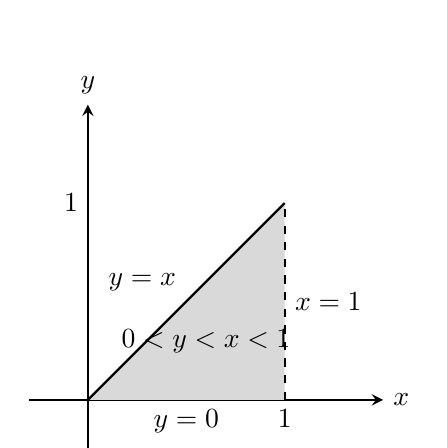
\begin{tikzpicture}[scale=2.5, >=stealth]
            % Axes
            \draw[->, thick] (-0.3, 0) -- (1.5, 0) node[right] {$x$};
            \draw[->, thick] (0, -0.3) -- (0, 1.5) node[above] {$y$};

            % Shaded Region
            \fill[gray!30] (0,0) -- (1,0) -- (1,1) -- cycle;

            % Boundary lines
            \draw[thick] (0,0) -- (1,1) node[midway, above left] {$y = x$};
            \draw[thick, dashed] (1,0) -- (1,1) node[midway, right] {$x = 1$};

            % Region Label
            \node at (0.6, 0.3) {$0 < y < x < 1$};

            % Axis Ticks & Labels
            \node[below] at (0.5, 0) {$y = 0$};
            \node[below] at (1, 0) {$1$};
            \node[left] at (0, 1) {$1$};
        \end{tikzpicture}
        \end{center}
    \end{list}
    \item Determine the normalizing constant $c$.
   \vspace{0.5em}
    \begin{list}{}{} \item[] 
        \textbf{Answer:}
        
        By edefinition, a valid joint probability random function must satisfy $\iint_{\mathcal{S}} f_{X,Y}(x,y) \, dA = 1$. Thus, integrating over $0 < y < x < 1$,
        \begin{align*}
        1 &= \int_{0}^{1} \int_{0}^{x} c(x + y) \, dy \, dx  \\
        &= c \int_{0}^{1} \left[ xy + \frac{y^2}{2} \right]_{y=0}^{y=x} \, dx  \\
        &= c \int_{0}^{1} \left( x^2 + \frac{x^2}{2} \right) \, dx  \\
        &= c \int_{0}^{1} \frac{3}{2}x^2 \, dx \\
        &= c \left[ \frac{1}{2}x^3 \right]_{0}^{1} = c \left( \frac{1}{2} \right).
        \end{align*}

        Setting $\frac{c}{2} = 1$. Therefore,
        \[        c = 2     \]
    \end{list}
    \item Derive the marginal densities $f_X(x)$ and $f_Y(y)$, including their supports.
    \vspace{0.5em}
    \begin{list}{}{} \item[] % Creates the indented answer block
        \textbf{Answer:}
        
        Note that $f_{X,Y}(x,y) = 2(x+y)$ on the nonrectangular support $0 < y < x < 1$ (where $c = 2$ from part b).

        \vspace{0.5em}
        \noindent By definition, the marginal probability random function of $X$ is
        \[
        f_X(x) = \int_{-\infty}^{\infty} f_{X,Y}(x,y) \, dy
        \]
        For $x \in (0, 1)$, the inequality $0 < y < x < 1$. Then,
        \begin{align*}
        f_X(x) &= \int_{0}^{x} 2(x + y) \, dy \\
        &= 2 \left[ xy + \frac{y^2}{2} \right]_{y=0}^{y=x} \\
        &= 2 \left( x(x) + \frac{x^2}{2} - 0 \right) \\
        &= 2 \left( \frac{3}{2}x^2 \right) = 3x^2.
        \end{align*}
        Therefore,
        \[
        f_X(x) = \begin{cases} 3x^2, & 0 < x < 1 \\ 0, & \text{otherwise} \end{cases}
        \]

        \vspace{0.5em}
        \noindent Similarly, the marginal probability random function of $Y$ is
        \[
        f_Y(y) = \int_{-\infty}^{\infty} f_{X,Y}(x,y) \, dx
        \]
        For $y \in (0, 1)$, the inequality is $0 < y < x < 1$. Then,
        \begin{align*}
        f_Y(y) &= \int_{y}^{1} 2(x + y) \, dx \\
        &= 2 \left[ \frac{x^2}{2} + xy \right]_{x=y}^{x=1} \\
        &= 2 \left[ \left( \frac{1^2}{2} + (1)y \right) - \left( \frac{y^2}{2} + y(y) \right) \right] \\
        &= 2 \left[ \frac{1}{2} + y - \frac{3}{2}y^2 \right] = 1 + 2y - 3y^2.
        \end{align*}
        Therefore,
        \[
        f_Y(y) = \begin{cases} 1 + 2y - 3y^2, & 0 < y < 1 \\ 0, & \text{otherwise} \end{cases}
        \]
    \end{list}
    \item Derive the conditional density $f_{Y \mid X}(y \mid x)$ and state its conditional support.
   \vspace{0.5em}
    \begin{list}{}{} \item[] 
        \textbf{Answer:}
        
        From the answer in (c), the conditional density function $f_{Y \mid X}(y \mid x)$ is 
        \[        f_{Y \mid X}(y \mid x) = \frac{f_{X,Y}(x,y)}{f_X(x)} \]
       Then, 
       \begin{align*}
        f_{Y \mid X}(y \mid x) &= \frac{f_{X,Y}(x,y)}{f_X(x)} \\
        &= \frac{2(x + y)}{3x^2} \\
        &= \frac{2}{3x} + \frac{2y}{3x^2}, 
        \end{align*}
        Therefore,
        \[ 
f_{Y \mid X}(y \mid x) = \begin{cases} \dfrac{2(x+y)}{3x^2}, & 0 < y < x \\ 0, & \text{otherwise} \end{cases} 
\]
    \end{list}
    \item Derive $\mathbb{E}(Y \mid X = x)$.
    \vspace{0.5em}
    \begin{list}{}{} \item[] 
        \textbf{Answer:}
        
        From the conditional probability density function derived in (d), $f_{Y \mid X}(y \mid x) = \dfrac{2(x+y)}{3x^2}$ for $0 < y < x$, $\mathbb{E}(Y \mid X = x)$ is 

        \begin{align*}
        \mathbb{E}(Y \mid X = x) &= \int_{-\infty}^{\infty} y f_{Y \mid X}(y \mid x) \, dy \\
        &= \int_{0}^{x} y \left( \frac{2(x+y)}{3x^2} \right) dy \\
        &= \frac{2}{3x^2} \int_{0}^{x} (xy + y^2) \, dy \\
        &= \frac{2}{3x^2} \left[ \frac{x y^2}{2} + \frac{y^3}{3} \right]_{y=0}^{y=x} \\
        &= \frac{2}{3x^2} \left( \frac{x(x^2)}{2} + \frac{x^3}{3} - 0 \right) \\
        &= \frac{2}{3x^2} \left( \frac{x^3}{2} + \frac{x^3}{3} \right) \\
        &= \frac{2}{3x^2} \left( \frac{5x^3}{6} \right) \\
        &= \frac{10 x^3}{18 x^2} = \frac{5}{9}x \quad 
        \end{align*}

        Therefore,
        \[        \mathbb{E}(Y \mid X = x) = \frac{5}{9}x \quad \text{for } 0 < x < 1.\]
    \end{list}
    \item Compute $\mathbb{E}(X)$, $\mathbb{E}(Y)$, and $\mathbb{E}(XY)$, and hence determine $\text{Cov}(X, Y)$.
    \vspace{0.5em}
    \begin{list}{}{} \item[] 
        \textbf{Answer:}
        
        \textbf{For $\mathbb{E}(X)$:} \\
        Using the marginal density $f_X(x) = 3x^2$ for $0 < x < 1$, then 
        \begin{align*}
        \mathbb{E}(X) &= \int_{0}^{1} x f_X(x) \, dx \\
        &= \int_{0}^{1} x (3x^2) \, dx \\
        &= \int_{0}^{1} 3x^3 \, dx \\
        &= \left[ \frac{3}{4}x^4 \right]_0^1 \\
        \mathbb{E}(X) &= \frac{3}{4}
        \end{align*}

        \textbf{For $\mathbb{E}(Y)$:} \\
        Using the marginal density $f_Y(y) = 1 + 2y - 3y^2$ for $0 < y < 1$, then
        \begin{align*}
        \mathbb{E}(Y) &= \int_{0}^{1} y f_Y(y) \, dy \\
        &= \int_{0}^{1} y (1 + 2y - 3y^2) \, dy \\
        &= \int_{0}^{1} (y + 2y^2 - 3y^3) \, dy \\
        &= \left[ \frac{y^2}{2} + \frac{2y^3}{3} - \frac{3y^4}{4} \right]_0^1 \\
        &= \frac{1}{2} + \frac{2}{3} - \frac{3}{4} \\
        &= \frac{6 + 8 - 9}{12} \\
        \mathbb{E}(Y) &= \frac{5}{12}
        \end{align*}

        \textbf{For $\mathbb{E}(XY)$:} \\
        Using the joint density $f_{X,Y}(x,y) = 2(x+y)$ over the support $0 < y < x < 1$, then
        \begin{align*}
        \mathbb{E}(XY) &= \int_{0}^{1} \int_{0}^{x} xy \cdot 2(x+y) \, dy \, dx \\
        &= 2 \int_{0}^{1} \int_{0}^{x} (x^2 y + x y^2) \, dy \, dx.
        \end{align*}
        Evaluating the inner integral first,
       \begin{align*}
        \int_{0}^{x} (x^2 y + x y^2) \, dy &= \left[ \frac{x^2 y^2}{2} + \frac{x y^3}{3} \right]_{y=0}^{y=x} \\
        &= \frac{x^4}{2} + \frac{x^4}{3} \\
        &= \frac{5x^4}{6}
        \end{align*}
        Evaluating the outer integral,
        \begin{align*}
        \mathbb{E}(XY) &= 2 \int_{0}^{1} \frac{5x^4}{6} \, dx \\
        &= \frac{5}{3} \int_{0}^{1} x^4 \, dx \\
        &= \frac{5}{3} \left[ \frac{x^5}{5} \right]_0^1 \\
        \mathbb{E}(XY) &= \frac{1}{3}
        \end{align*}

        \textbf{For $\text{Cov}(X, Y)$:} \\
        By definition of covariance,
        \[
        \text{Cov}(X, Y) = \mathbb{E}(XY) - \mathbb{E}(X)\mathbb{E}(Y).
        \]
        Hence,
        \begin{align*}
        \text{Cov}(X,Y) &= \frac{1}{3} - \left( \frac{3}{4} \right) \left( \frac{5}{12} \right) \\
        &= \frac{1}{3} - \frac{15}{48} \\
        &= \frac{16}{48} - \frac{15}{48} \\
        &= \frac{1}{48}
        \end{align*}
        Therefore,
        \[
        \text{Cov}(X, Y) = \frac{1}{48}.
        \]
    \end{list}
    \item Determine whether $X$ and $Y$ are independent. Give two separate arguments: one based on the support and one based on the factorization criterion.
    \vspace{0.5em}
    \begin{list}{}{} \item[] % Creates the indented answer block
        \textbf{Answer:}
        
        
        For $X$ and $Y$ to be independent, $f_{X,Y}(x,y) = f_X(x) \cdot f_Y(y)$ must hold for all $(x,y)$.

        Note that from (c), 
        \[
        f_X(x) = 3x^2 \quad \text{and} \quad f_Y(y) = 1 + 2y - 3y^2 \quad \text{on } (0,1).
        \]
     
        Hence, the product $f_X(x)f_Y(y)$ is
        \begin{align*}
        f_X(x)f_Y(y) &= 3x^2 (1 + 2y - 3y^2) \\
        f_X(x)f_Y(y) &= 3x^2 + 6x^2y - 9x^2y^2.
        \end{align*}
        Note that,
        \[        f_{X,Y}(x,y) = 2(x+y) = 2x + 2y.        \]
        Hence, $3x^2 + 6x^2y - 9x^2y^2 \neq 2x + 2y$. \\
        Moreover, the support $0 < y < x < 1$ is triangular (nonrectangular). Thus, the bounds of $y$ depend on $x$.\\
        Therefore, $X$ and $Y$ are dependent.
    \end{list}
\end{enumerate}

\vspace{1.5em}

\subsection*{Problem 4. Zero Correlation and Dependence \hfill \mdseries[10 points]}

Let
\[
X \sim \text{Uniform}(-1, 1),
\]
and define
\[
Y = X^2.
\]

\begin{enumerate}[(a)]
    \item Derive $\mathbb{E}(X)$, $\mathbb{E}(Y)$, and $\mathbb{E}(XY)$ from the distribution of $X$.
    \item Show that $\text{Cov}(X, Y) = 0$.
    \item Prove that $X$ and $Y$ are not independent. Your proof may not rely solely on the statement ``$Y$ is a function of $X$''; use a probability or conditional-distribution argument.
    \item Explain, in no more than four mathematically precise sentences, why zero correlation fails to imply independence in this example.
\end{enumerate}

\vspace{1.5em}

\subsection*{Problem 5. A Non-One-to-One Transformation \hfill \mdseries[14 points]}
Let
\[X \sim \text{Uniform}(0, 1)\]
and define
\[Y = X(1 - X).\]
\begin{enumerate}[(a)]
    \item Determine the support of $Y$.
    \vspace{0.5em}
    \begin{list}{}{} \item[] % Creates the indented answer block
        \textbf{Answer:}
        
        Let $X \sim U(0, 1)$, then the probability density function of $X$ is
        \[        f_X(x) = \begin{cases} 1, & \text{if } 0 < x < 1, \\ 0, & \text{if otherwise.} \end{cases}\]
        Define $Y = X(1 - X)$. Since $0 < x < 1$, then
        \[        0 < x(1 - x) < \frac{1}{4}        \]
        Therefore,
        \[        0 < y < \frac{1}{4}        \]
    \end{list}
    \item Show that the transformation $y = x(1 - x)$ is not one-to-one on $(0, 1)$, and obtain all inverse branches $x = x(y)$.
    \vspace{0.5em}
    \begin{list}{}{} \item[] % Creates the indented answer block
        \textbf{Answer:}
        
        From
        \begin{align*}
        y &= x(1 - x) \\
        y &= x - x^2
        \end{align*}
        Solving for $x$ in terms of $y$, then
        \begin{align*}
        y &= x - x^2 \\
        x^2 - x + y &= 0
        \end{align*}
        Thus,
        \[        x = \frac{1 \pm \sqrt{1 - 4y}}{2} .       \]
        Therefore, the two inverse branches are
        \[        x_1(y) = \frac{1 + \sqrt{1 - 4y}}{2} \quad \text{and} \quad x_2(y) = \frac{1 - \sqrt{1 - 4y}}{2}
        \]
    \end{list}
    \item Using the CDF method, derive $F_Y(y)$ for all real $y$. Your derivation must explicitly account for both inverse branches.
    \vspace{0.5em}
    \begin{list}{}{} \item[] % Creates the indented answer block
        \textbf{Answer:}
        
        From the branches,
        \[        x < x_1(y) \quad \text{or} \quad x > x_2(y)        \]
        Then,
        \[        F_Y(y) = P(x < x_1(y)) + P(x > x_2(y))        \]
        Since $f_X(x) = 1$ for $0 < x < 1$, then
        \[        F_Y(y) = x_1(y) + [1 - x_2(y)]        \]
        Thus substituting the branches,
        \begin{align*}
        F_Y(y) &= \frac{1 + \sqrt{1 - 4y}}{2} + \left[ 1 - \frac{1 - \sqrt{1 - 4y}}{2} \right] \\
        &= 1 - \sqrt{1 - 4y}
        \end{align*}
        Therefore,
        \[        F_Y(y) = \begin{cases} 0, & y \le 0 \\ 1 - \sqrt{1 - 4y}, & 0 < y < \dfrac{1}{4} \\ 1, & y \ge \dfrac{1}{4} \end{cases}
        \]
    \end{list}
    \item Differentiate the CDF to obtain $f_Y(y)$, including its support.
   
\vspace{0.5em}
    \begin{list}{}{} \item[] 
        \textbf{Answer:}
        
        Differentiate $F_Y(y)$ with respect to $y$:
        \begin{align*}
        f_Y(y) &= \frac{d}{dy} \left[ 1 - \sqrt{1 - 4y} \right] \\
        &= -\frac{1}{2} (1 - 4y)^{-\frac{1}{2}} (-4) \\
        f_Y(y) &= \frac{2}{\sqrt{1 - 4y}}
        \end{align*}
        Therefore,
        \[
        f_Y(y) = \begin{cases} \dfrac{2}{\sqrt{1 - 4y}}, & 0 < y < \dfrac{1}{4} \\ 0, & \text{otherwise} \end{cases}
        \]
    \end{list}    
    \item Verify independently that your derived PDF integrates to $1$.
    \vspace{0.5em}
    \begin{list}{}{} \item[] 
        \textbf{Answer:}
        
        By integrating the probability density function $f_Y(y)$ over its support $\left(0, \frac{1}{4}\right)$:
        \begin{align*}
        \int_{0}^{\frac{1}{4}} \frac{2}{\sqrt{1 - 4y}} \, dy &= \left[ -\sqrt{1 - 4y} \right]_0^{\frac{1}{4}} \\
        &= -\sqrt{1 - 4\left(\frac{1}{4}\right)} - \left[ -\sqrt{1 - 4(0)} \right] \\
        &= -\sqrt{0} - (-\sqrt{1}) \\
        \int_{0}^{\frac{1}{4}} \frac{2}{\sqrt{1 - 4y}} \, dy &= 1
        \end{align*}
        Therefore,
        \[        \int_{0}^{\frac{1}{4}} \frac{2}{\sqrt{1 - 4y}} \, dy = 1
        \]
    \end{list}
    \item Compute $\mathbb{E}(Y)$ directly from $\mathbb{E}[g(X)]$. Then compute $\mathbb{E}(Y)$ again using your derived density $f_Y$ and verify that the two answers agree.
    \vspace{0.5em}
    \begin{list}{}{} \item[] % Creates the indented answer block
        \textbf{Answer:}

        Let $X$ have probability density function
        \[        f_X(x) = \begin{cases} 1, & 0 < x < 1, \\ 0, & \text{elsewhere.} \end{cases}
        \]
        Let $Y = g(X) = X(1 - X) = X - X^2$.

        \vspace{0.5em}
        By the Law of the Unconscious Statistician , the expectation of $Y = g(X) = X(1 - X)$ is given by
        \[\mathbb{E}(Y) = \mathbb{E}[g(X)] = \int_{-\infty}^{\infty} g(x) f_X(x) \, dx\]
        Then,
        \noindent Evaluating $E(X)$:
        \begin{align*}
        E(X) &= \int_{0}^{1} x(1) \, dx \\
        &= \left[ \frac{x^2}{2} \right]_0^1 \\
        &= \frac{1^2}{2} - \frac{0^2}{2}  \\
        &= \frac{1}{2}
        \end{align*}

        \noindent Evaluating $E(X^2)$:
        \begin{align*}
        E(X^2) &= \int_{0}^{1} x^2(1) \, dx \\
        &= \left[ \frac{x^3}{3} \right]_0^1 \\
        &= \frac{1^3}{3} - \frac{0^3}{3} \\
        &= \frac{1}{3}
        \end{align*}
      \noindent From the Linearity of Expectation,
        \[E(X - X^2) = E(X) - E(X^2).\]
        Then,
        \begin{align*}
        E(X - X^2)  &= \frac{1}{2} - \frac{1}{3} \\
        E(X - X^2)  &= \frac{1}{6}
        \end{align*}

        \vspace{1em}
        Let $Y$ have the derived probability density function
        \[        f_Y(y) = \begin{cases} \dfrac{2}{\sqrt{1 - 4y}}, & 0 < y < \dfrac{1}{4}, \\ 0, & \text{elsewhere.} \end{cases}
        \]

        \vspace{0.5em}
        From the definition of Expected value of a continuous random variable, 
        \[
        \mu = E(Y) = \int_{-\infty}^{\infty} y f_Y(y) \, dy
        \]

        \noindent Then,
        \[
        E(Y) = \int_{0}^{\frac{1}{4}} y \left( \frac{2}{\sqrt{1 - 4y}} \right) dy
        \]
       Let $u = \sqrt{1 - 4y}$ (where $u^2 = 1 - 4y \implies y = \frac{1 - u^2}{4}$ and $du = -\frac{2}{\sqrt{1 - 4y}} \, dy \implies \left(\frac{2}{\sqrt{1 - 4y}}\right) dy = -du$), with bounds $y = 0 \to u = 1$ and $y = \frac{1}{4} \to u = 0$. Then,
        \begin{align*}
        E(Y) &= \int_{1}^{0} \left( \frac{1 - u^2}{4} \right) (-du)
        \end{align*}
        Thus, by reversing the bounds of integration,
        \begin{align*}
        E(Y) &= \int_{0}^{1} \frac{1 - u^2}{4} \, du \\
        &= \frac{1}{4} \left[ u - \frac{u^3}{3} \right]_0^1 \\
        &= \frac{1}{4} \left( 1 - \frac{1}{3} \right) - \frac{1}{4} \left( 0 - \frac{0}{3} \right) \\
        &= \frac{1}{4} \left( \frac{2}{3} \right) \\
        &= \frac{1}{6}
        \end{align*}

        Since $E(Y) = \dfrac{1}{6}$. Therefore, the two methods of computing $\mathbb{E}(Y)$ agree.
    \end{list}
\end{enumerate}

\vspace{1.5em}

\subsection*{Problem 6. Multivariate Transformation and Jacobian \hfill \mdseries[16 points]}

Let $X$ and $Y$ be independent random variables with densities
\[f_X(x) = \frac{x^{\alpha-1} e^{-x}}{\Gamma(\alpha)}, \quad x > 0,\]
\[f_Y(y) = \frac{y^{\beta-1} e^{-y}}{\Gamma(\beta)}, \quad y > 0,\]
where $\alpha > 0$ and $\beta > 0$. Define the transformation
\[U = X + Y, \quad V = \frac{X}{X + Y}.\]

\begin{enumerate}[(a)]
    \item Solve for $x$ and $y$ as functions of $u$ and $v$.
    \vspace{0.5em}
    \begin{list}{}{} \item[] % Creates the indented answer block
        \textbf{Answer:}
        
        Define the transformation
        \[        U = X + Y, \quad V = \frac{X}{X + Y}.        \]
        Then,
        \[        V = \frac{X}{X + Y}        \]
        Since $U = X + Y$, then 
        \[        v = \frac{x}{u}        \]
        \[        x = u v        \]
        From $U = X + Y$, substituting $x = u v$ then
        \[        u = u v + y        \]
        Hence,
        \begin{align*}
        y &= u - u v \\
        y&= u(1 - v)
        \end{align*}
        Therefore,
        \[        x(u,v) = uv \quad \text{and} \quad y(u,v) = u(1-v).        \]
    \end{list}
    \item Determine the transformed support of $(U, V)$ directly from $x > 0$ and $y > 0$.
    \vspace{0.5em}
    \begin{list}{}{} \item[] % Creates the indented answer block
        \textbf{Answer:}
        
        From (a), the inverse transformations are $x = uv$ and $y = u(1-v)$.
        
        Since $U = X + Y$ and $X > 0$ and $Y > 0$, then
        \[        u = x + y > 0        \]
        From $x > 0$, substitute $x = uv$. Thus,
        \begin{align*}
        x > 0 &\implies uv > 0 \\
        &\implies \frac{1}{u}(uv > 0) \\
        &\implies v > 0
        \end{align*}
        From $y > 0$, substitute $y = u(1-v)$. Then,
        \begin{align*}
        y > 0 &\implies u(1-v) > 0 \\
        &\implies \frac{1}{u}(u(1-v) > 0) \\
        &\implies 1 - v > 0 \\
        &\implies v < 1
        \end{align*}
        Therefore,
        \[        u > 0 \quad \text{and} \quad 0 < v < 1.        \]
    \end{list}
    \item Compute the Jacobian determinant
    \[    \left| \frac{\partial(x, y)}{\partial(u, v)} \right|    \]
    from the derivative matrix.
     \vspace{0.5em}
    \begin{list}{}{} \item[] % Creates the indented answer block
        \textbf{Answer:}
        
        Note that from (a), $x(u,v) = uv$ and $y(u,v) = u(1-v)$.
        Then,
        \[        \begin{pmatrix} \dfrac{\partial x}{\partial u} & \dfrac{\partial x}{\partial v} \\[0.8em] \dfrac{\partial y}{\partial u} & \dfrac{\partial y}{\partial v} \end{pmatrix} = \begin{pmatrix} v & u \\ 1-v & -u \end{pmatrix}
        \]
        From the Jacobian determinant $J = \dfrac{\partial(x,y)}{\partial(u,v)}$, then
        \begin{align*}
        J &= \det \begin{pmatrix} v & u \\ 1-v & -u \end{pmatrix} \\
        &= (v)(-u) - (u)(1-v) \\
        &= -uv - u + uv \\
        J &= -u
        \end{align*}
        Therefore,
        \begin{align*}
            |J| &= |-u| \\
            |J| & = u 
        \end{align*}
    \end{list}
    \item Derive the joint density $f_{U,V}(u, v)$, including the support.
    \vspace{0.5em}
    \begin{list}{}{} \item[] % Creates the indented answer block
        \textbf{Answer:}
        
        Since $X$ and $Y$ are independent random variables, the joint probability density function is
        \[
        f_{X,Y}(x,y) = f_X(x) \cdot f_Y(y) = \frac{x^{\alpha-1} e^{-x}}{\Gamma(\alpha)} \cdot \frac{y^{\beta-1} e^{-y}}{\Gamma(\beta)} = \frac{x^{\alpha-1} y^{\beta-1} e^{-(x+y)}}{\Gamma(\alpha)\Gamma(\beta)} \quad \text{for } x > 0, y > 0
        \]
        Hence, the joint probability density function of $(U, V)$ is 
        \[
        f_{U,V}(u,v) = f_{X,Y}\big(x(u,v), y(u,v)\big) \cdot |J|
        \]
        Note that from (a), $x = uv$ and $y = u(1-v)$. Then,
       \begin{align*}
    f_{X,Y}(uv, u(1-v)) &= \frac{x^{\alpha-1} y^{\beta-1} e^{-(x+y)}}{\Gamma(\alpha)\Gamma(\beta)} \cdot |J| \\
    &= \frac{(uv)^{\alpha-1} [u(1-v)]^{\beta-1} e^{-[uv + u(1-v)]}}{\Gamma(\alpha)\Gamma(\beta)} \cdot |J| \\
    &= \frac{u^{\alpha+\beta-2} v^{\alpha-1} (1-v)^{\beta-1} e^{-u}}{\Gamma(\alpha)\Gamma(\beta)} \cdot |J|\\
    f_{X,Y}(uv, u(1-v)) &= \frac{u^{\alpha+\beta-2} v^{\alpha-1} (1-v)^{\beta-1} e^{-u}}{\Gamma(\alpha)\Gamma(\beta)} \cdot |J|
    \end{align*}
    
        From (c), the $|J| = u$. Then,
        \begin{align*}
        f_{U,V}(u,v) &= \left( \frac{u^{\alpha+\beta-2} v^{\alpha-1} (1-v)^{\beta-1} e^{-u}}{\Gamma(\alpha)\Gamma(\beta)} \right) \cdot u \\
        &= \frac{u^{\alpha+\beta-1} e^{-u}}{\Gamma(\alpha)\Gamma(\beta)} \, v^{\alpha-1} (1-v)^{\beta-1}
        \end{align*}
        Therefore,
        \[        f_{U,V}(u,v) = \begin{cases} \dfrac{u^{\alpha+\beta-1} e^{-u}}{\Gamma(\alpha)\Gamma(\beta)} \, v^{\alpha-1} (1-v)^{\beta-1}, & u > 0 \text{ and } 0 < v < 1 \\[1em] 0, & \text{otherwise} \end{cases}
        \]
    \end{list}
    \item Derive the marginal density of $U$ and identify its distribution.
    \item Derive the marginal density of $V$ and identify its distribution.
    \item Determine whether $U$ and $V$ are independent. Justify your conclusion by factorizing the joint density, not by inspection alone.
    \item Specialize your result to $\alpha = \beta = 1$. What is the distribution of $V$ in this case? Explain why this agrees with your general result.
\end{enumerate}

\vspace{1.5em}

\subsection*{Problem 7. Order Statistics from First Principles \hfill \mdseries[14 points]}

Let $X_1, X_2, \dots, X_n$ be independent and identically distributed continuous random variables with common CDF $F$ and PDF $f$. Define
\[
X_{(1)} = \min(X_1, \dots, X_n), \quad X_{(n)} = \max(X_1, \dots, X_n).
\]

\begin{enumerate}[(a)]
    \item Starting from the event $\{X_{(n)} \le x\}$, derive the CDF and PDF of $X_{(n)}$. Do not quote a memorized order-statistic formula.
    \item Starting from the event $\{X_{(1)} > x\}$, derive the CDF and PDF of $X_{(1)}$.
    \item For $a < b$, derive
    \[
    P(X_{(1)} > a, X_{(n)} < b)
    \]
    in terms of $F(a)$ and $F(b)$. State any continuity assumptions you use.
    \item Now suppose $X_1, \dots, X_n \sim \text{Uniform}(0, \theta)$, where $\theta > 0$. Derive the PDFs of $X_{(1)}$ and $X_{(n)}$ explicitly.
    \item For the $\text{Uniform}(0, \theta)$ case, derive $\mathbb{E}[X_{(n)}]$ from its density.
    \item Find a constant $k_n$, depending only on $n$, such that
    \[
    \mathbb{E}[k_n X_{(n)}] = \theta.
    \]
    Derive $k_n$ rather than guessing it.
\end{enumerate}

\vspace{1.5em}

\subsection*{Problem 8. Proof Critique and Repair \hfill \mdseries[6 points]}

Consider the following argument about two random variables $X$ and $Y$:

\begin{quote}
``Since $\text{Cov}(X, Y) = 0$, $X$ and $Y$ are independent. Therefore
\[
f_{X,Y}(x, y) = f_X(x) f_Y(y),
\]
and consequently
\[
\mathbb{E}[XY] = \mathbb{E}[X] \mathbb{E}[Y].
\]
''
\end{quote}

\begin{enumerate}[(a)]
    \item Identify the first logically invalid implication in the argument and explain precisely why it is invalid.
    \item Using the random variables in Problem 4, provide a counterexample to the invalid implication.
    \item State a correct sufficient condition under which
    \[
    f_{X,Y}(x, y) = f_X(x) f_Y(y)
    \]
    holds.
    \item Rewrite the original argument as a logically valid implication chain under an appropriate assumption.
\end{enumerate}

\end{document}


